\documentclass[tikz,border=6pt]{standalone}
\usepackage{amsmath,amssymb}
\usetikzlibrary{shapes.geometric,positioning,decorations.pathreplacing,calc}

\begin{document}
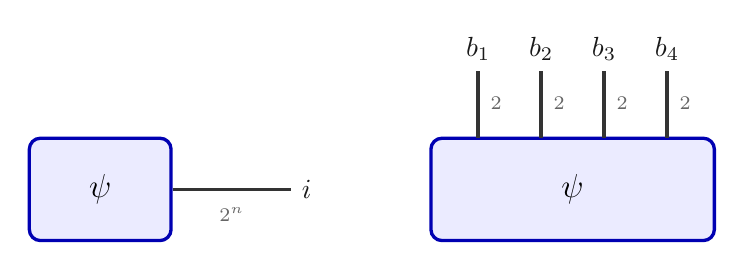
\begin{tikzpicture}[
    tensor/.style={draw=blue!70!black, fill=blue!8, rounded corners=4pt, line width=1.2pt, minimum height=1.3cm, align=center},
    leg/.style={line width=1.3pt, draw=black!80},
    dimlabel/.style={font=\scriptsize\color{black!60}},
    indexlabel/.style={font=\normalsize\color{black!90}}
]

    % --- Left: Vector representation ---
    \begin{scope}[xshift=0cm]
        \node[tensor, minimum width=1.8cm] (vec) at (0, 0) {\large $\psi$};
        \draw[leg] (vec.east) -- ++(1.5, 0) node[right, indexlabel] {$i$};
        \node[dimlabel, below=3pt] at ($(vec.east) + (0.75, 0)$) {$2^n$};
    \end{scope}

    % --- Right: Tensor representation ---
    \begin{scope}[xshift=4.5cm]
        \node[tensor, minimum width=3.6cm] (ten) at (1.5, 0) {\large $\psi$};
        
        % Legs
        \foreach \x/\lbl in {0.3/b_1, 1.1/b_2, 1.9/b_3, 2.7/b_4} {
            \draw[leg] (\x, 0.65) -- (\x, 1.5) node[above, indexlabel] {$\lbl$};
            \node[dimlabel, right=1pt] at (\x, 1.1) {2};
        }
    \end{scope}

\end{tikzpicture}
\end{document}
